%-----------------RUTH AND LINDELO-----------------
\subsection{Platform}
\begin{itemize}
		\item Java EE
	\begin{itemize}
		\item 
	\end{itemize}
\end{itemize}

\subsection{Frameworks}
\begin{itemize}
		\item Java Server Faces
	\begin{itemize}
		\item 
	\end{itemize}
\end{itemize}
	
	
\subsection{Databases}
\subsubsection{Relational Databases}
\begin{itemize}
	\item MySQL Database
	\begin{itemize}
	\item 
	\end{itemize}
\end{itemize}
	
\subsubsection{Object Relational Databases}
\begin{itemize}
	\item Postgresql
	\begin{itemize}
	\item 
	\end{itemize}
\end{itemize}

\subsubsection{NoSQL Databases}
\begin{itemize}
	\item Neo4j
	\begin{itemize}
	\item 
	\end{itemize}
%	\item The Scalability discussed here can be seen as an illustration in Figure ~\ref{fig:scalability}.
%	\begin{figure}[H]
%		\centering
%		\fbox{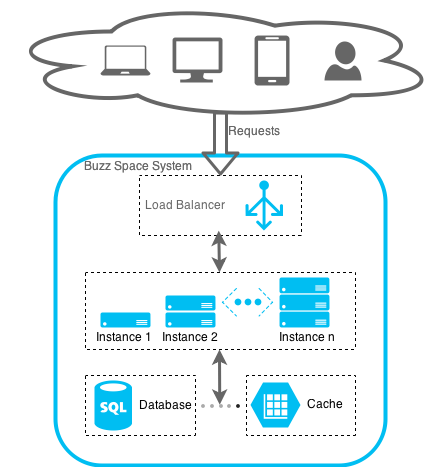
\includegraphics[width=1.0\textwidth]{Scalability.png}}
%		\caption{How the system architecture can be set-up to allow many concurrent connections.}
%		\label{fig:scalability}
%	\end{figure}
\end{itemize}

\subsection{Object Relational Mappers}
\begin{itemize}
	\item Hibernate Query Language
	\begin{itemize}
	\item Great for working with Java
	\item Can query any database
	\end{itemize}
\end{itemize}

\subsection{Languages}
\subsubsection{Programming Languages}
\begin{itemize}
	\item JavaScript
	\begin{itemize}
	\item 
	\end{itemize}
	
	\item Java
	\begin{itemize}
	\item 
	\end{itemize}
\end{itemize}

\subsubsection{Mark-up Languages}
\begin{itemize}
	\item HTML
	\begin{itemize}
	\item hi
	\end{itemize}
\end{itemize}


\subsection{Application Servers}
\begin{itemize}
	\item GlassFish Server
	\begin{itemize}
	\item 
	\end{itemize}

	\item Tomcat
	\begin{itemize}
	\item 
	\end{itemize}


\end{itemize}

\subsection{Dependency Management}
\begin{itemize}
	\item Apache Maven
	\begin{itemize}
	\item Works well with Java
	\end{itemize}

\end{itemize}

\subsection{Web Services}
\begin{itemize}
	\item SOAP-based
	\begin{itemize}
	\item 
	\end{itemize}

\end{itemize}
